\documentclass[]{article}

%opening
\title{MLP Coursework 3}
\author{Eskil Joergensen}
\date{\today}

\usepackage[parfill]{parskip}
\usepackage{pgfgantt}
\usepackage{multicol}
\usepackage{tikz}
\usepackage{pgfplots}

\usepackage{graphicx}
\graphicspath{ {images/} }

\usepackage{amsmath}

\usepackage{booktabs}
\usepackage[font={small,it}]{caption}

\begin{document}

\maketitle

\section{Introduction}


The report aims to investigate, present and discuss three simple questions:
How does the choice of activation function affect the performance of a multi-layer neural network? How does the number of hidden layer and hidden units affect the training of a deep neural network? Can a learning rate scheduler increase the performance of a simple feed-forward network? Using a simple model, CIFAR-10 image classification and TensorFlow, a number of small experiments related to the training of deep neural networks.


\section{Methodology}

As the methodology used for the three experiments were similar, this section will cover the overall structure of the code and neural networks used throughout the investigation. Instead of building three isolated models and corresponding methods to run the experiments, some effort was put into building a system that would accommodate all the intended trials. 

By looping over arrays of experimental parameters, the actual experiments were easily controlled and initiated once the necessary code was in place. 

\subsection{The Core Model}

A simple three-layer model, interleaved with non-linear transformations, was chosen as a basis for this study. 

To investigate the aforementioned questions, only specific aspects of the model, or training procedure, were changed during the experimentation. The weights for the fully connected layers were initialized by a random distribution, using the \texttt{tf.truncated\_normal} function from TensorFlow. Then the biases are initialized with \texttt{tf.zeros} to ensure they start with all zero values, and their shape is simply the number of units in the layer to which they connect. A simple schematic representation of the model can be seen in Figure \ref{part1-model}.

The model was trained on image classification, using labeled images from the CIFAR-10 data set. To accommodate the CIFAR-10 image size of 32x32, and three color channels, the model's input dimension was 3x32x32. Furthermore the base model had 200 hidden units in the hidden layers, and a 10 dimensional output layer (10 classes). A cross entropy error function was used with the model, which was implemented using  \texttt{softmax\_cross\_entropy\_with\_logits} from TensorFlow.

\begin{figure}[h]
	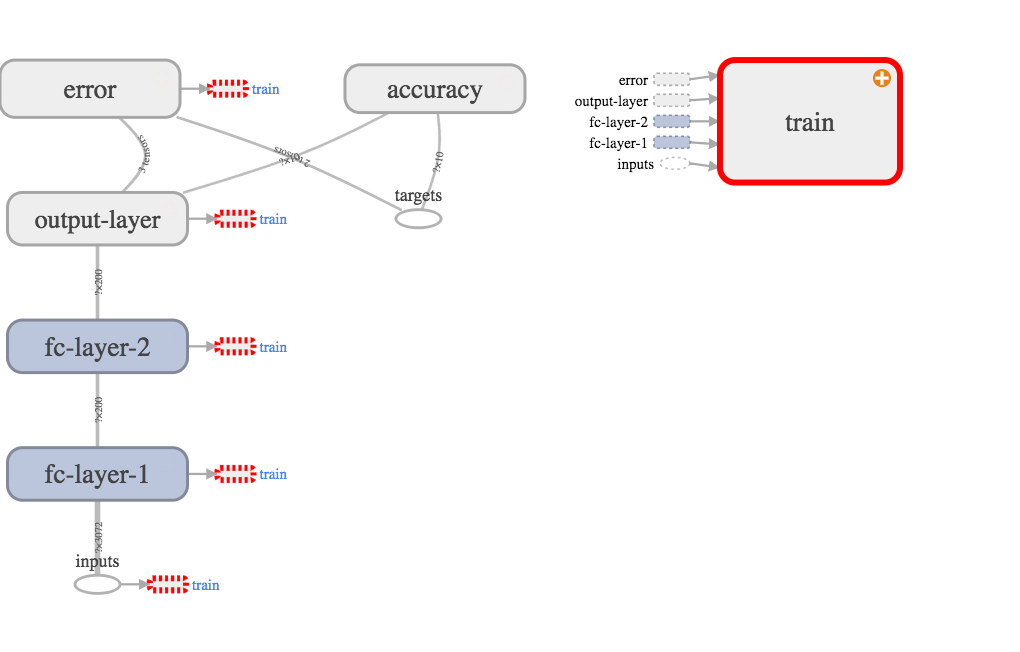
\includegraphics[width=\textwidth]{model_1}
	\caption{Showing a visual representation of the model used, from TensorBoard.}
	\label{part1-model}
	\centering
\end{figure}

\subsection{The Training}

The model was trained for 40 epochs, or 32,000 steps, with batch size of 50, in all three experiments. The \texttt{AdamOptimizer} was used as the default optimizer, with a learning rate of 0.01. The Summary Operator from TensorFlow was used to record the data from the experiments. The training data was recorded every step, whereas the validation data was recorded every 100 steps.

\subsection{The Experiments}


\subsubsection{Activation Functions}

Four activation functions were compared. The logistic sigmoid $f(x)=\frac{1}{1+e^{-x}}$, the hyperbolic tangent $f(x)=tanh(x)$ the rectified linear (ReLu) $f(x)=max(0,x)$ and the exponential linear unit (ELU):

\begin{equation} \label{eq:elu}
f(x) = \begin{cases}
x &\text{if $x >$ 0}\\ \alpha (\text{exp}(x) - 1) &\text{if  $x \leq$ 0}
\end{cases}
\end{equation}

where \(\alpha\) is a hyperparameter that decides the range of negative values for which the activation function saturates.

\begin{figure}[h]
	\centering
	\begin{tikzpicture}
	\begin{axis}[
	width=0.4\textwidth,
	axis lines = left,
	xlabel = $x$,
	ylabel = {$f(x)$},
	xmin=-4, xmax=4,
	ymin=-2, ymax=3,
	]
	\addplot[color=red]{max(0, x)};
	\end{axis}
	\end{tikzpicture}
	\begin{tikzpicture}
	\begin{axis}[
	width=0.4\textwidth,
	axis lines = left,
	xlabel = $x$,
	ylabel = {$f(x)$},
	xmin=-4, xmax=4,
	ymin=-2, ymax=3,
	]
	\addplot[color=blue]{tanh(x)};
	\end{axis}
	\end{tikzpicture}
	\begin{tikzpicture}
	\begin{axis}[
	width=0.4\textwidth,
	axis lines = left,
	xlabel = $x$,
	ylabel = {$f(x)$},
	xmin=-4, xmax=4,
	ymin=-2, ymax=3,
	]
	\addplot[color=brown]{1/(1+e^(-x))};
	\end{axis}
	\end{tikzpicture}
	\begin{tikzpicture}
	\begin{axis}[
	width=0.4\textwidth,
	axis lines = left,
	xlabel = $x$,
	ylabel = {$f(x)$},
	xmin=-4, xmax=4,
	ymin=-2, ymax=3,
	]
	\addplot[color=green, domain=-4:0]{e^(x)-1};
	\addplot[color=green, domain=0:4]{x};
	\end{axis}
	\end{tikzpicture}
	\caption{Showing the plots of the activation functions. Top Left: Relu. Top Right: Tanh. Bottom Light: Sigmoid. Bottom Right: ELU}
	\label{part1-plots}
\end{figure}

Both the hyperbolic tangent and the sigmoid functions compress their input values between (-1, 1) and (0, 1) respectively. A result of such saturation will cause their gradients to approach zero, which means smaller parameter changes and slower training. Two key differences between the two are that the hyperbolic tangent allows for both positive and negative outputs, and that the hyperbolic tangent is centered around zero. The sigmoid transformation function is centered around 0.5, which may not be ideal.

The ReLu transformation function looks and behaves quite differently from the two before mentioned alternatives, see Figure \ref{part1-plots}. The ReLu function has a constant gradient of 1 for activations greater than zero, and it will not suffer from diminishing gradients. It can however kill all the units, by responding to everything with 0. Furthermore, as it is unbounded, it will be more sensitive to learning rates than the sigmoid and hyperbolic tangent.

In addition to ReLu, the Exponential Linear Unit (ELU), was also tested. Although their   Unlike ReLU, the ELU responds to negative values, which pushes the mean of the activations closer to zero. Mean activations that are closer to zero enable faster learning as they bring the gradient closer to the natural gradient  \cite{elu}.

The four activation functions were used in turn to train the three-layer model presented above. The only difference, the new activation function would override the default (ReLu) non-linearity. 

\subsubsection{Hidden Layers}

The second experiment involved investigating how the arrangement of hidden layers and hidden units would effect the performance of the training of a model. A series of depths and widths were tested using two nested loops. 

The main obstruction was creating a system that would dynamically allocate the desired number of hidden layers in the model. A dictionary was used to store the fully connected layers by their respective TensorFlow name scope identifiers. As the number of hidden units was the same for all the hidden layers, it was easily implemented. 

A number of combinations of hidden units and layers were integrated into the base model. The number of hidden layers tested in the model were 1, 2 and 4, combined with 50, 100, 200 and 400 hidden units. 

\subsubsection{Learning Rate Schedules}

The third experiment investigates the implementation of a time-dependent learning rate schedule. This report uses an exponential learning rate schedule  
\begin{equation} \label{eq:1}
\eta(t) = \eta_{0} \gamma ^{(t / t_{decay})}
\end{equation}
where \(\eta(t)\) is the learning rate after t steps, \(\eta_{0}\) the initial learning rate and \(\gamma\) is the decay rate. \(t_{decay}\) is the number of steps required for one decay-cycle. The value of \(\gamma\) and \(t_{decay}\) determine the rate of decay of the learning rate. For the learning rate experiments, the \texttt{GradientDescentOptimizer} replaced the Adam optimizer.

The learning schedule was implemented using already built functionality from TensorFlow. In addition to minimizing the training error, the optimizer can also be used to control the learning rate, see Figure \ref{model_2}. The optimizer iterates over the steps taken, which changes the learning rate as the training progresses. TensorFlow offers a number of learning rate schedulers, in this investigation the exponential version, \texttt{tf.train.exponential\_decay}, was used. 

\begin{figure}[h]
	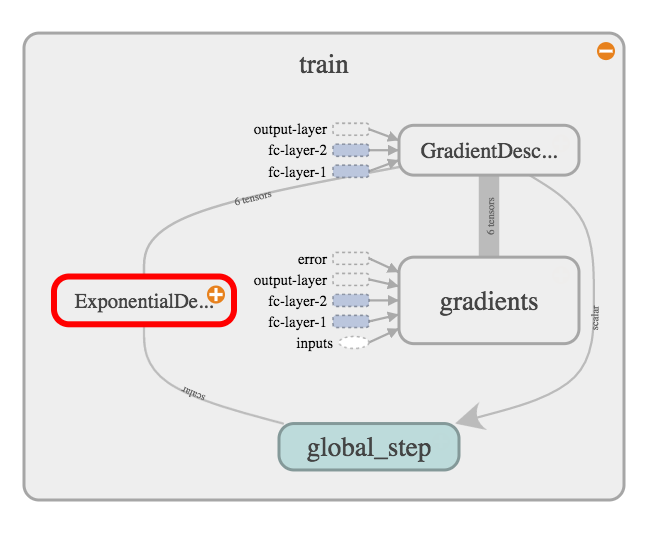
\includegraphics[width=\textwidth]{model_2}
	\caption{Showing a schematic representation of how the learning rate is updated within the graph, from TensorBoard.}
	\label{model_2}
	\centering
\end{figure}

The decay rate and the decay steps were only changed during some initial testing, and were set to 0.96 and 10,000 respectively. The initial learning rates used were 0.005, 0.02, 0.025, 0.03, 0.05, 0.07 and 0.1. 

\section{Results and Discussion}

\subsection{Activation Functions}

After the model was trained with all the activation functions, the ELU performed significantly better than the other activation functions, see Figure \ref{res-activ}. The final classification error for ELU was 0.96, whereas the hyperbolic tangent performed worst, with a final classification error of 1.58. The training with ReLu and sigmoid showed similar results. 


\begin{figure}[h]
	\centering
	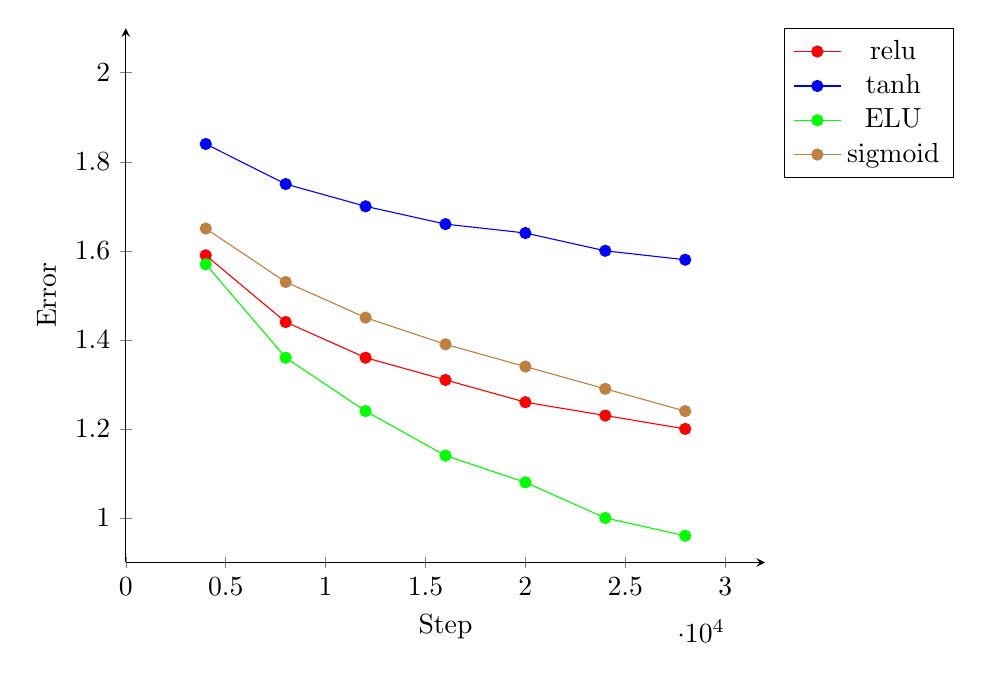
\begin{tikzpicture}
	\begin{axis}[
	width=0.8\textwidth,
	axis lines = left,
	xlabel = {Step},
	ylabel = {Error},
	xmin=0, xmax=32000,
	ymin=0.9, ymax=2.1,
	legend pos=outer north east
	]
		\addplot[color=red,mark=*]
	coordinates {
		(4000, 1.59)(8000, 1.44)(12000, 1.36)(16000, 1.31)(20000, 1.26)(24000, 1.23)(28000, 1.2)
	};
	\addlegendentry{relu};
	\addplot[color=blue,mark=*]
	coordinates {
	(4000, 1.84)(8000, 1.75)(12000, 1.7)(16000, 1.66)(20000, 1.64)(24000, 1.6)(28000, 1.58)
	};
	\addlegendentry{tanh};
	\addplot[color=green,mark=*]
	coordinates {
	(4000, 1.57)(8000, 1.36)(12000, 1.24)(16000, 1.14)(20000, 1.08)(24000, 1.0)(28000, 0.96)
};
	\addlegendentry{ELU};
	
	\addplot[color=brown,mark=*]
	coordinates {
	(4000, 1.65)(8000, 1.53)(12000, 1.45)(16000, 1.39)(20000, 1.34)(24000, 1.29)(28000, 1.24)
};
	\addlegendentry{sigmoid};
	
	\end{axis}
	\end{tikzpicture}
	
	\caption{Showing the evolution of the error function values across the training steps, for the different activation functions.}
	\label{res-activ}
\end{figure}

\begin{table}[]
	\centering
	\caption{Displaying the final classification accuracies for the activation functions.}
	\label{part1-table}
	\begin{tabular}{@{}lcc@{}}
		\toprule
		\multicolumn{1}{c}{} & Final training set accuracy & Final validation set accuracy \\ \midrule
		ELU & 0.669 & 0.505 \\
		ReLu & 0.553 & 0.483 \\
		Sigmoid & 0.537 & 0.481 \\
		Tanh & 0.472 & 0.401 \\ \bottomrule
	\end{tabular}
\end{table}

The results from the training errors are also reflected in the final classification accuracies, see Table \ref{part1-table}. The ReLu and the sigmoid performed very similarly. Having to choose between the two is more difficult, but taking into account that the ReLu is computationally more efficient, that should break the tie. However, in other scenarios with different models or learning rules, an initial trial using both non-linear functions is advisable.

Based on the results presented here, it is clear that the ELU activation function outperformed the other three. As the first use of the ELU was published quite recently, it is interesting to see how well it performs. Although the network used in this experiment was quite simple, the findings are consistent with those of the original publishers \cite{elu}. 

\subsection{Hidden layers}

For the second experiment, the results were mostly very similar. In the case of a single hidden layer, no interesting level of learning was observed. With a classification accuracy around 0.08, the three trials with a single hidden layer (the non-deep networks) were dismissed. 

Besides the one outsider, the training data shows a very similar performance for remaining five configurations. The two best trials were both from the models with three hidden layers, see Figure \ref{res-hidden}.

\begin{figure}[h]
	\centering
	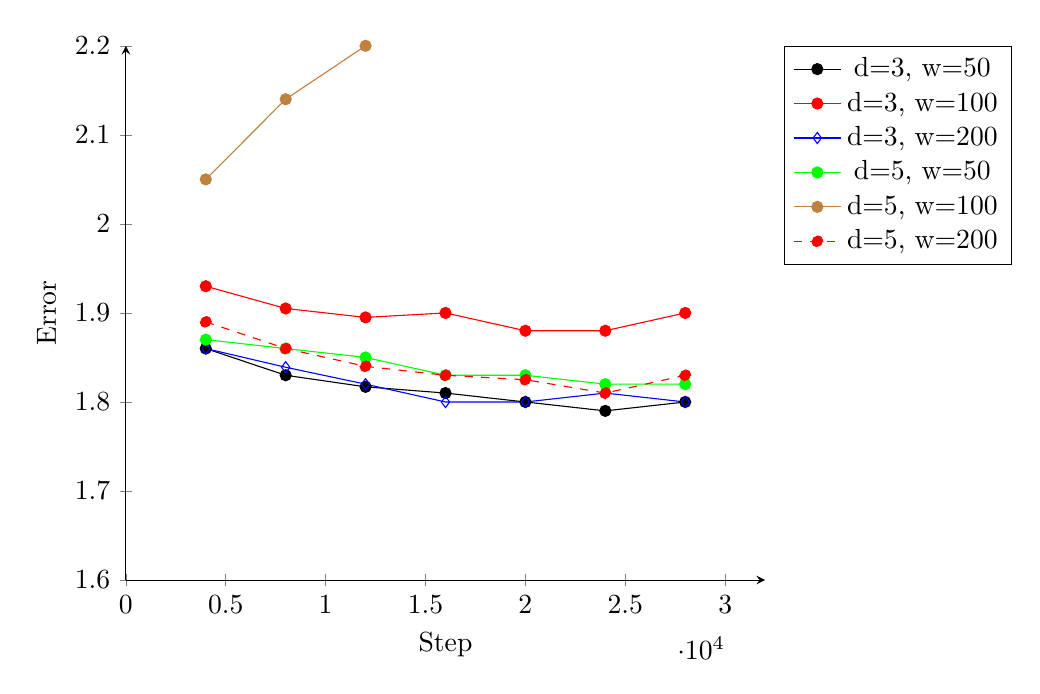
\begin{tikzpicture}
	\begin{axis}[
	width=0.8\textwidth,
	axis lines = left,
	xlabel = {Step},
	ylabel = {Error},
	xmin=0, xmax=32000,
	ymin=1.6, ymax=2.2,
	legend pos=outer north east
	]
	\addplot[color=black,mark=*]
	coordinates {
		(4000, 1.86)(8000, 1.83)(12000, 1.817)(16000, 1.81)(20000, 1.8)(24000, 1.79)(28000, 1.8)
	};
	\addlegendentry{d=3, w=50};
	\addplot[color=red,mark=*]
	coordinates {
		(4000, 1.93)(8000, 1.905)(12000, 1.895)(16000, 1.9)(20000, 1.88)(24000, 1.88)(28000, 1.9)
	};
	\addlegendentry{d=3, w=100};
	\addplot[color=blue,mark=diamond]
	coordinates {
		(4000, 1.86)(8000, 1.839)(12000, 1.82)(16000, 1.8)(20000, 1.8)(24000, 1.81)(28000, 1.8)
	};
	\addlegendentry{d=3, w=200};
	\addplot[color=green,mark=*]
	coordinates {
		(4000, 1.87)(8000, 1.86)(12000, 1.85)(16000, 1.83)(20000, 1.83)(24000, 1.82)(28000, 1.82)
	};
	\addlegendentry{d=5, w=50};
	\addplot[color=brown,mark=*]
	coordinates {
		(4000, 2.05)(8000, 2.14)(12000, 2.2)(16000, 2.24)(20000, 2.29)(24000, 2.3)(28000, 2.304)
	};
	\addlegendentry{d=5, w=100};
	\addplot[dashed, color=red,mark=*]
	coordinates {
		(4000, 1.89)(8000, 1.86)(12000, 1.84)(16000, 1.83)(20000, 1.825)(24000, 1.81)(28000, 1.83)
	};
	\addlegendentry{d=5, w=200};
	\end{axis}
	\end{tikzpicture}
	
	\caption{Showing the evolution of the error function values across the training steps, for different depths and widths of the hidden layers.}
	\label{res-hidden}
\end{figure}

Even though the results may indicate better performance using fewer hidden layers, one must realize that additional hidden layers, may require other changes in the network or training process to benefit from the additional layers. 

\subsection{Learning Rate Schedules}

Seven initial learning rates were tested. However, as the trials for 0.02, 0.025 and 0.03 were visually identical, the results from 0.02 and 0.03 have been omitted from this section. Figure \ref{res-sch} shows the relevant findings.

The results show that the training with the initial learning rate of 0.025 and 0.05 performed significantly better than the other initial learning rates (besides 0.02 and 0.03). As the error increases for learning rates lower than 0.025, as well as for learning rates over 0.05, it seems plausible that the optimal initial learning rate lies between 0.025 and 0.05 for the current model. 


\begin{figure}[h]
	\centering
	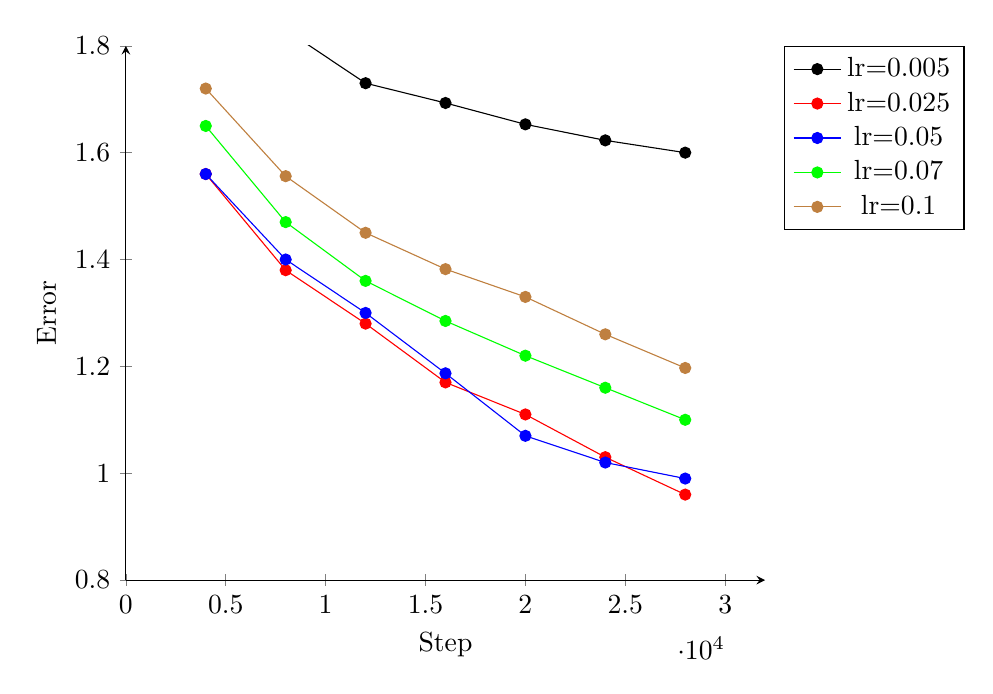
\begin{tikzpicture}
	\begin{axis}[
	width=0.8\textwidth,
	axis lines = left,
	xlabel = {Step},
	ylabel = {Error},
	xmin=0, xmax=32000,
	ymin=0.8, ymax=1.8,
	legend pos=outer north east
	]
	\addplot[color=black,mark=*]
	coordinates {
		(4000, 1.93)(12000, 1.73)(16000, 1.693)(20000, 1.653)(24000, 1.623)(28000, 1.6)
	};
	\addlegendentry{lr=0.005};
	\addplot[color=red,mark=*]
	coordinates {
		(4000, 1.56)(8000, 1.38)(12000, 1.28)(16000, 1.17)(20000, 1.11)(24000, 1.03)(28000, 0.96)
	};
	\addlegendentry{lr=0.025};
	\addplot[color=blue,mark=*]
	coordinates {
		(4000, 1.56)(8000, 1.4)(12000, 1.3)(16000, 1.187)(20000, 1.07)(24000, 1.02)(28000, 0.99)
	};
	\addlegendentry{lr=0.05};
	\addplot[color=green,mark=*]
	coordinates {
		(4000, 1.65)(8000, 1.47)(12000, 1.36)(16000, 1.285)(20000, 1.22)(24000, 1.16)(28000, 1.1)
	};
	\addlegendentry{lr=0.07};
	
	\addplot[color=brown,mark=*]
	coordinates {
		(4000, 1.72)(8000, 1.556)(12000, 1.45)(16000, 1.382)(20000, 1.33)(24000, 1.26)(28000, 1.197)
	};
	\addlegendentry{lr=0.1};
	
	\end{axis}
	\end{tikzpicture}
	
	\caption{Showing the evolution of the error function values across the training steps, for some of the initial learning rates.}
	\label{res-sch}
\end{figure}

\section{Conclusion}

In conclusion, the results of this investigation were not revolutionary. Although the reason behind the simple feed-forward model was to more easily observe changes in performance, it may have been too simplistic. However, experimenting with the ELU activation function was interesting, and it will be interesting to see if will be adopted by the community. 

Despite the lack of new revelations, having set up a system that allows for a versatile and dynamic way to set up and train models, may help further experimentation in the future. 

\section{Future Work}

Following on the progress and findings of this investigation, the next step involves building on the current setup so it can handle more complex scenarios. Initially a procedure for setting up and running convolutional neural networks will be implemented. Secondly, other complimentary features like drop out and max pooling are still needed, and will be even more relevant with convolutional neural networks. 

Lastly, some investigation will go into the use of ELU as a part of a convolutional neural network. 

\clearpage
\medskip
\bibliographystyle{IEEEtran}
\bibliography{ref.bib}

\end{document}
